\subsection{Redes neurais convolucionais}

Uma rede neural convolucional é análoga à rede neural artificial, i.e., feita de neurônios que otimizam o aprendizado através dele mesmo. A principal diferença é que a rede neural convolucional é amplamente utilizada em soluções que detectam padrões em imagens, logo existem funcionalidades específicas da própria arquitetura para essa tarefa \cite{oshea2015introduction}. 

Uma arquitetura básica de uma rede neural convolucional tem as seguintes camadas: convolucional, agrupamento e totalmente conectada \cite{dp_overview}.

\begin{figure}[H]
	\caption{Camadas principais de uma rede neural convolucional}
	\centering % para centralizarmos a figura
	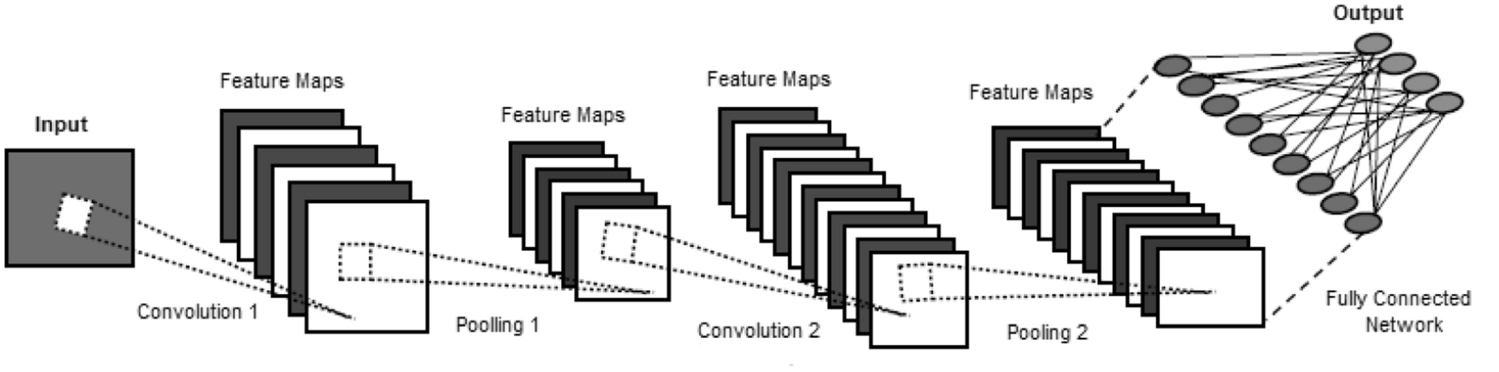
\includegraphics[width=15cm]{figures/arquitetura_cnn.png} % leia abaixo
	\legend{Fonte: \citeonline{dp_overview}}
	\label{fig:arquitetura_cnn}
\end{figure}

\subsubsection*{Camada convolucional}

Segundo \citeonline{computation11030052} camada convolucional é essencial para esse tipo de arquitetura e usa um filtro — ou kernel — para aplicar na imagem e direcionar para o próximo neurônio. Esse filtro é uma matriz de números que terá uma operação aplicada em todos os píxeis da imagem — que também é representado por matriz(es) — as informações cruciais para esse filtro são: tamanho, largura e pesos. Isto é utilizado para extrair características com uma base matemática, criando uma relação direta entre um píxel e os píxeis ao redor. Os pesos começam de forma pseudoaleatórias e são ajustados no decorrer do aprendizado. O resultado dessa camada é chamado de mapa de características. O tamanho da saída será baseado na fórmula abaixo sendo os tamanhos I da imagem, F do filtro e a S da saída \cite{computation11030052}.

\begin{gather}
    \mathbf{I}x - \mathbf{F}x + 1 = \mathbf{S}x \notag \\
    \mathbf{I}y - \mathbf{F}y + 1 = \mathbf{S}y
\end{gather}

    
A seguir um exemplo dos passos para construir a matriz resultante baseado em \citeonline{Alzubaidi2021}.

$$
\hspace{0.4cm}
\begin{tikzpicture}[baseline=(M.center)]
 \matrix (M) [matrix of math nodes,left delimiter={[},right delimiter={]}] {
 0 & 2 & 1 & 0 \\
 1 & 0 & 0 & 1 \\
 };
 \draw (M-1-1.north west) rectangle (M-2-2.south east);
 \node[above=10pt of M.north] {Matriz 2x4};
\end{tikzpicture}
\hspace{0.8cm}\bigotimes\hspace{0.8cm}
\begin{tikzpicture}[baseline=(M.center)]
 \matrix (M) [matrix of math nodes,left delimiter={[},right delimiter={]}] {
  0 & 1 \\
 -1 & 2 \\
 };
 \node[above=10pt of M.north] {Filtro 2x2};
\end{tikzpicture}
\hspace{0.8cm}=\hspace{0.8cm}
\begin{tikzpicture}[baseline=(M.center)]
 \matrix (M) [matrix of math nodes,left delimiter={[},right delimiter={]}] {
    \boxed{1} & - & - \\
 };
 \node[above=10pt of M.north] {Resultado};
\end{tikzpicture}
$$

$$
\begin{tikzpicture}[baseline=(M.center)]
 \matrix (M) [matrix of math nodes,left delimiter={[},right delimiter={]}] {
    0 & 2 & 1 & 0 \\
    1 & 0 & 0 & 1 \\
 };
 \draw (M-1-2.north west) rectangle (M-2-3.south east);
\end{tikzpicture}
\hspace{0.8cm}\bigotimes\hspace{0.8cm}
\begin{tikzpicture}[baseline=(M.center)]
 \matrix (M) [matrix of math nodes,left delimiter={[},right delimiter={]}] {
  0 & 1 \\
  -1 & 2 \\
 };
\end{tikzpicture}
\hspace{0.8cm}=\hspace{0.8cm}
\begin{bmatrix}
 1 & \boxed{1} & - \\
 \end{bmatrix}
$$

$$
\hspace{0.2cm}
\begin{tikzpicture}[baseline=(M.center)]
 \matrix (M) [matrix of math nodes,left delimiter={[},right delimiter={]}] {
    0 & 2 & 1 & 0 \\
    1 & 0 & 0 & 1 \\
 };
 \draw (M-1-3.north west) rectangle (M-2-4.south east);
\end{tikzpicture}
\hspace{1cm}\bigotimes\hspace{0.9cm}
\begin{tikzpicture}[baseline=(M.center)]
 \matrix (M) [matrix of math nodes,left delimiter={[},right delimiter={]}] {
  0 & 1 \\
  -1 & 2 \\
 };
\end{tikzpicture}
\hspace{0.8cm}=\hspace{0.8cm}
\begin{bmatrix}
 1 & 1 &  \boxed{2} \\
 \end{bmatrix}
$$

\subsubsection*{Tamanho do passo e preenchimento}

O Tamanho do passo — ou stride — serve para especificar a distancia de pixels entre os passos da camada.  No exemplo acima esse parâmetro é definido como 1, por isso a matriz selecionada pula 1 pixel para direita entre os passos. Esse valor altera o tamanho da matriz resultante \cite{dp_overview}.

O preenchimento — ou padding — é uma técnica utilizada para manter o mesmo tamanho da entrada, adicionando bordas com zeros antes das operações da camada para ter como saída uma matriz da mesma dimensão da matriz original. Isso é usado devido a desvantagem em perder os detalhes nas bordas das imagens no processamento de uma camada \cite{dp_overview}.

\subsubsection*{Camada de agrupamento}

A camada de agrupamento — ou pooling — tem como tarefa primordial uma técnica para reduzir o tamanho do mapa de características, porém preservando os padrões mais relevantes. Dentre os recursos essenciais dessa camada estão o tamanho do agrupamento e a operação que será realizada. O maior problema dessa camada é pelo fato dela apenas identificar onde essas características estão e não se tem ou não, \emph{i.e.}, dependendo de qual operação e a quantidade de camadas pode não ser possível guardar as principais características de forma integra causando uma redução no desempenho final da predição \cite{dp_overview}.

Existem vários tipos de agrupamento, os mais utilizados são: agrupamento máximo, agrupamento médio e agrupamento global médio que estão explicados abaixo em exemplos baseados em \citeonline{Alzubaidi2021}.

\subsubsubsection*{Agrupamento máximo}

É definido o resultado com base no máximo encontrado pelo tamanho do agrupamento, exemplo a seguir usando um mapa de características com tamanho 4x4 e agrupamento de tamanho 2x2.

$$
\begin{tikzpicture}[baseline=-0.5ex]
    \matrix (M) [matrix of math nodes,left delimiter={[},right delimiter={]}] {
        4 & 25 & 44 & 10\\
        8 & 14 & 8 & 33 \\
        17 & 2 & 16 & 34 \\
        5 & 13 & 24 & 7 \\
    };
    \draw (M-1-1.north west) rectangle (M-2-2.south east);
\end{tikzpicture}
= 
\begin{bmatrix}
	\boxed{25} & 44 \\
	17 & 34 \\
   \end{bmatrix}
$$

\subsubsubsection*{Agrupamento médio}

É definido o resultado com base na média encontrada pelo tamanho do agrupamento, exemplo a seguir usando um mapa de características com tamanho 4x4 e agrupamento de tamanho 2x2.

$$
\begin{tikzpicture}[baseline=-0.5ex]
    \matrix (M) [matrix of math nodes,left delimiter={[},right delimiter={]}] {
        4 & 25 & 44 & 10\\
        8 & 14 & 8 & 33 \\
        17 & 2 & 16 & 34 \\
        5 & 13 & 24 & 7 \\
    };
    \draw (M-1-1.north west) rectangle (M-2-2.south east);
\end{tikzpicture}
= 
\begin{bmatrix}
	\boxed{12} & 23 \\
	9 & 20 \\
   \end{bmatrix}
$$

\subsubsubsection*{Agrupamento global médio}

É definido o resultado com base na média geral do mapa o que sempre tem como saída uma matrix 1x1, exemplo a seguir usando um mapa de características com tamanho 4x4.

$$
\begin{tikzpicture}[baseline=-0.5ex]
    \matrix (M) [matrix of math nodes,left delimiter={[},right delimiter={]}] {
        4 & 25 & 44 & 10\\
        8 & 14 & 8 & 33 \\
        17 & 2 & 16 & 34 \\
        5 & 13 & 24 & 7 \\
    };
\end{tikzpicture}
= 
\begin{bmatrix}
	16
   \end{bmatrix}
$$

\subsubsection*{Camada totalmente conectada}

A camada totalmente conectada geralmente é utilizada no final da arquitetura e cria a partir de cada neurônio uma ligação direta para cada etiqueta final. Isso torna essa camada extremamente pesada computacionalmente. O número de neurônios dessa camada é equivalente ao número de classes propostas. Além disso é quando chega nessa camada que a função de perda é calculada e se inicia a retropropagação \cite{Alzubaidi2021, computation11030052}.

\subsubsection*{Aperfeiçoamento}

Segundo \citeonline{Alzubaidi2021, computation11030052} existem algumas técnicas para aperfeiçoar os resultados do modelo, sendo elas:

\begin{itemize}
    \item Dropout: Muito utilizada para evitar sobreajuste pois está técnica irá desligar um neurônio aleatoriamente colocando a saída dele como zero no processo de treinamento e portanto forçara o modelo a aprender a identificar características diferentes em outros neurônios possibilitando a generalização do modelo.
    \item Aumentar o tamanho do conjunto de dados: caso não seja possível criar ou encontrar um maior existem técnicas para aumentar artificialmente acrescentando pequenas mudanças nas imagens existentes, algumas são rotacionar, recortar e inverter horizontalmente ou verticalmente.
    \item Normalização em lote: normaliza os pesos para evitar o problema de mudança interna de covariância
    \item Aumentar o tempo de treinamento
    \item Aumentar a profundidade ou largura da arquitetura
    \item Ajustar os hiperparâmetros
\end{itemize}
    